\chapter{Risk Management}

Il risk management è il processo che consiste nell'identificare, analizzare e valutare il rischio. Si tratta dell'unico modo per assicurare che i controlli di cybersecurity scelti siano appropriati ai rischi che l'organizzazione affronta. Senza risk assessment ad informare le scelte di cybersecurity, c'è il rischio di sprecare tempo, sforzo e risorse. Ha poco senso infatti implementare misure di sicurezza contro minacce improbabili che accadano o che abbiano impatto materiale limitato sull'organizzazione, senza contare che vi è il rischio di sottostimare o ignorare rischi che potrebbero effettivamente colpire l'organizzazione. 

Le organizzazioni devono decidere quanto tempo e denaro spendere proteggere la loro tecnologia e i loro servizi. Uno degli obiettivi principali della gestione del rischio è quello di informare e migliorare queste decisioni. In base al settore in cui l'azienda opera, il risk management può essere un obbligo. Ad esempio, un'organizzazione che vuole la certificazione ISO 27001, avere una strategia di risk management è uno dei requisiti chiave (è richiesto anche da GDPR).
\\

\noindent Un processo di risk management si compone di più fasi:
\begin{itemize}
    \item Nella fase iniziale, l'azienda che lo mette in atto deve definire la strategia per il risk management, dove vengono definiti la metodologia usata dall'azienda, le componenti essenziali dell'organizzazione che ne devono essere soggette (es: informazione, processi che elaborano i servizi), chi sono gli stakeholders del sistema;
    \item Nella fase cardine, quella di risk assessment, si identificano, analizzano e valutano i rischi;
    \item Nella fase di Risk Treatment l'organizzazione, per ciascun dei rischi individuati, vengono identificate le misure di protezione. In questa fase non bisogna tenere presente solo il rischio però, ma anche le risorse disponibili (economiche, personale, ...). Alla fine del processo esisterà sempre un rischio minimo che non è stato mitigato. L'azienda dovrà quindi decidere se accettare il rischio, per continuare a fornire i suoi servizi, monitorare il rischio in attesa di cambiamenti oppure trasferire il rischio a terzi (assicurazione);
    \item I rischi identificati vanno infine comunicati agli stakeholder del sistema;
    \item Nella fase di monitor and review le misure di protezione selezionate e implementatevengono monitorate per garantire che forniscano sempre un livello di protezione adeguato rispetto agli attacchi identificati nella fase di risk assessment. Questo può essere fatto con penetration testing o valutando le performance delle misure adottate intervistando gli stakeholders. In base al risultato di questa fase, potrebbe essere necessario ripartire da capo. L'attività di revisione del rischio può anche essere fatta qualora l'azienda decide di introdurre nuove funzionalità/sistemi o raccogliere nuove informazioni. Ad esempio, se l'azienda decide di spostare i dati dei clienti dai server locale a un servizio cloud, è necessario rifare il processo da capo
\end{itemize}

\noindent Il processo di risk management è un processo ciclico.

\section{Standard NIST}

Il NIST fornisce uno standard per le fase di risk management viste. Il vantaggio di usare gli standard del NIST è che sono open-surce.

\noindent Tra gli standard che fornisce troviamo:
\begin{itemize}
    \item Lo standard 800-39 che ci dà un'introduzione generale ai concetti alla base del processo di information management;
    \item Lo standard 800-37 che ci descrive come implementare un programma di risk management;
    \item Lo standard 800-30 che ci descrive il processo di risk assessment;
    \item Lo standard 800-53 che riguarda la fase di risk treatment;
    \item Lo standard 800-53a che descrive come valutare l'efficacia dei security controls identificati nella fase di risk treatment;
    \item Lo standard 800-39 che descrive come classificare le informazioni per il risk assessment, se il focus dell'azienda consiste in quelle;
\end{itemize}

\noindent Oltre gli standard del NIST ne esistono altri:
\begin{itemize}
    \item ISO/IEC IS 27005 che fornisce un processo generale per il risk management, non legato specificatamente alla sicurezza;
    \item ISO 31000, un altro standard generale;
    \item Altre metodologie nazionali.
\end{itemize}

\noindent Esistono anche metodologie legate solo al risk assessment: OCTAVE, CORAS (basata solo su grafici),  EBIOS, CRAMM, ...

\subsection{Modellazione del rischio}
Quando parliamo di rischio dobbiamo definire i fattori che andiamo ad usare per quantificare il rischio. Quasi tutte le metodologie parlano di rischio rispetto all'asset. Gli asset contengono vulnerabilità. I threat actor iniziano uno o più threat event che vanno a creare un threat scenario, un attacco che consiste di più fasi. 

Il rischio è dato da due componenti: la probabilità che avvenga e l'impatto che questo potrebbe avere su uno o più asset dell'organizzazione. 

Vediamo uno scenario generico: il rischio si materializza quando abbiamo un threat agent che inizia un attacco sfruttando delle vulnerabilità che risulta in un impatto negativo per l'organizzazione. Il rischio viene dato dall'impatto negativo e dalla likelihood. Questa è composta dalla probabilità che l'attacco avvenga e dalla probabilità che questo ha di impattare (\ref{fig:11-4}). 

\begin{figure}
    \centering
    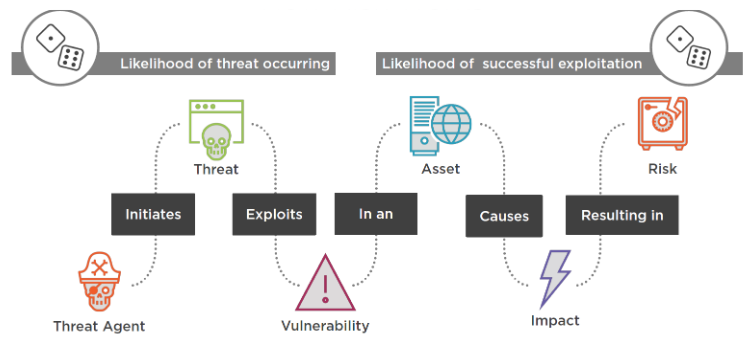
\includegraphics[width=0.8\textwidth]{images/11-8.png}
    \caption{Modello di rischio.}
    \label{fig:11-4}
\end{figure}

\paragraph{OWASP Risk Rating Methodology} Fornisce una serie di fattori per stimare la probabilità e l'impatto. La probabilità è stimata sulla base di due serie di fattori:
\begin{itemize}
    \item Fattori dell'agente di minaccia;
    \item Fattori di vulnerabilità.
\end{itemize}
\noindent L'impatto è stimato sulla base di:
\begin{itemize}
    \item Fattori di impatto tecnico;
    \item Fattori di impatto sul business.
\end{itemize}

\section{Risk assessment secondo lo standard NIST}

Supponiamo di avere Poste Italiane che permette di eseguire operazione di online bancking, sia tramite app online che app da cellulare. Le informazione vengono memorizzate da un online bancking service, a cui le due app accedono. Per accedere ai servizi, i clienti devono utilizzare un username e una password.

Per identificare i rischi di questo scenario usiamo il risk assessment definito nello standard NIST 800-30. Lo standard si compone di 4 fase:
\begin{enumerate}
    \item Raccolta di tutti documenti necessari per fare l'analisi del rischio;
    \item Identificazione dei rischi e valutazione della loro severità in base alla likelihood;
    \item Comunicazione dei risultati del risk assessment al CEO, CESO e manager, che decidono quali rischi mitigare;
    \item Revisione periodica del risk assessment, per adeguarlo ai cambiamenti.
\end{enumerate}

\subsection{Preparazione al risk assessment}
L'obiettivo di questa fase è definire il contesto per il risk assessment. Si compone di quattro task:
\begin{enumerate}
    \item Se determina il perché si sta facendo l'assessment. Esistono due possibilità:
    \begin{itemize}
        \item Si tratta del primo assessment. Vogliamo stabilire una baseline dei possibili attacchi e conseguenti rischi (attaccanti, vulnerabilità, come possono essere sfruttate le vulnerabilità, ...);
        \item Stiamo revisionando un assessment precedente per revisionare i rischi a cui è soggetto l'organizzazione. Viene fatto per due motivi:
        \begin{itemize}
            \item Lo scenario è cambiato, sono emersi nuovi attacchi a cui è soggetta l'organizzazione (es: è stata scoperta la vulnerabilità log4j);
            \item è stata rilasciata una nuova applicazione, o una precedente è stata ad esempio rilasciata su cloud, e vogliamo valutare quali sono i rischi associati. 
        \end{itemize}
    \end{itemize}

    \item Si definisce lo scope dell'assessment, ovvero quali parti dei sistemi gestiti dall'organizzazione sono soggetti al risk assessment (target dell'analisi - app sul cloud, determinate informazione e servizi associati);

    \item Si documentano quali sono le assunzioni fatte relative all'analisi. Bisogna recuperare qual è la strategia aziendale rispetto al risk assessment. Questa comprende la risk tolerance (rischio che l'organizzazione è disposta a tollerare sopo che le misure di protezione identificate dal risk assessment sono state implementate) e risk acceptance. Si definiscono anche la metodologia per effettuare il risk assessment e quali sono le categorie di attaccanti, attacchi e vulnerabilità rilevanti per l'organizzazione. Si definiscono infine i valori da usare per quantificare la likelihood di un attacco e dei possibili impatti negativi che possono verificarsi;

    \item Si definisce il risk model, ovvero i fattori che usiamo per quantificare il rischio (generalmente i modelli usano threat, vulnerability, ...). Si valuta anche l'approccio per valutare il rischio. Esistono tre approcci principali:
    \begin{itemize}
        \item Approccio qualitativo: si esprime la probabilità dell'impatto usando delle etichette come probabilità alta, media, bassa o impatto alto, medio, moderato;
        \item Approccio quantitativo: likelihood e impatto vengono espressi numericamente;
        \item Approccio ibrido: usa i numeri per quantificare il valore associato a likelihood e impatto e presenta tali risultati poi con delle etichette. SI definisce infine l'approccio di analisi. Questo dipende dalla metodologia che si utilizza (alcune metodologie di risk assessment partono dall'asset e risalgono a tutti i possibili attacchi o che partano dall'individuare i possibili attaccanti e legano le possibili categorie trovate agli asset del sistema).
    \end{itemize}
\end{enumerate}

\begin{figure}
    \centering
    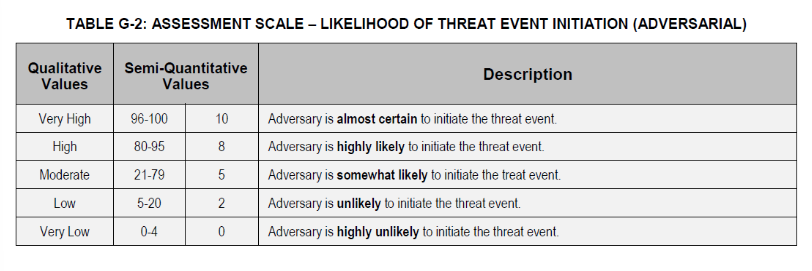
\includegraphics[width=1\textwidth]{images/11-1.png}
    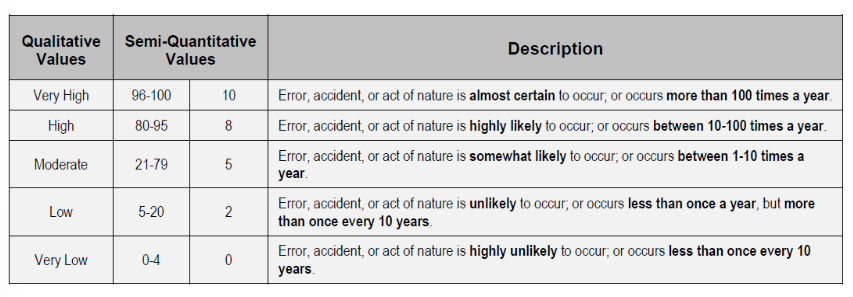
\includegraphics[width=1\textwidth]{images/11-2.png}
    \caption{Tabelle NIST likelihood singolo.}
    \label{fig:11-1}
\end{figure}

\begin{figure}
    \centering
    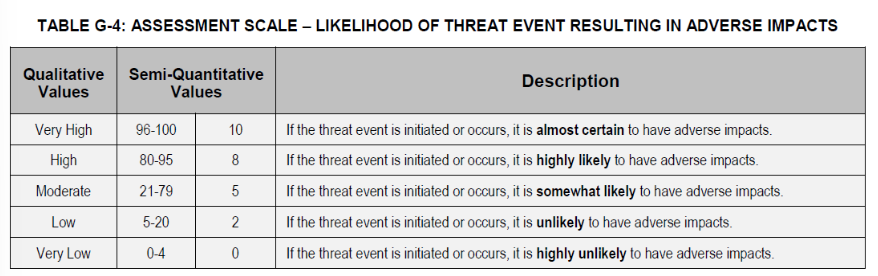
\includegraphics[width=1\textwidth]{images/11-3.png}
    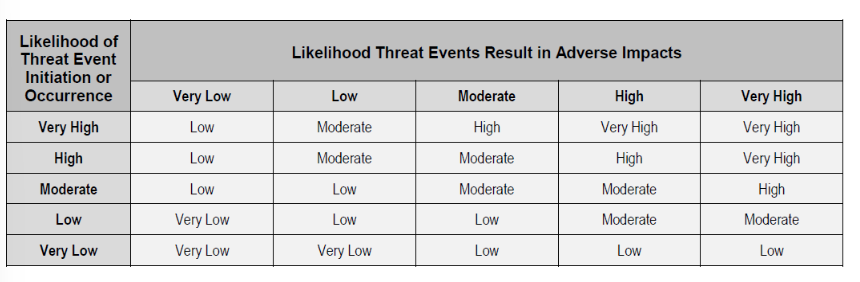
\includegraphics[width=1\textwidth]{images/11-4.png}
    \caption{Tabelle NIST likelihood congiunto.}
    \label{fig:11-5}
\end{figure}

\begin{figure}
    \centering
    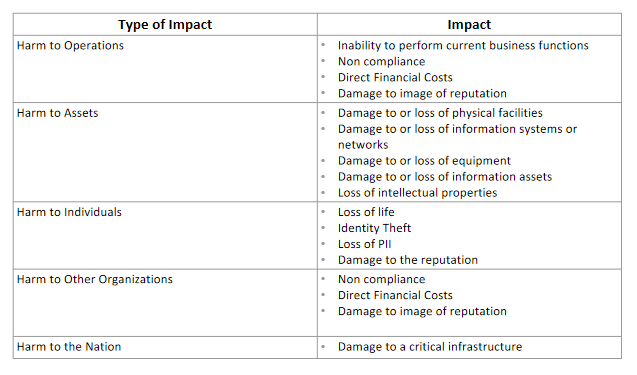
\includegraphics[width=0.9\textwidth]{images/11-5.png}
    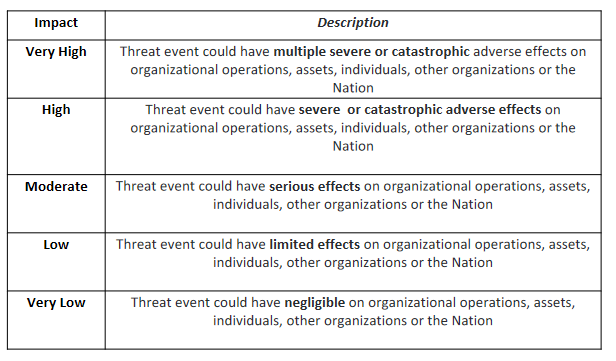
\includegraphics[width=0.9\textwidth]{images/11-6.png}
    \caption{Tabelle NIST impatto.}
    \label{fig:11-2}
\end{figure}

\subsection{Esecuzione del risk assessment}
L'obiettivo di questa fase è produrre una lista di possibili attacchi col proprio livello di rischio, ordinati per tale livello (quelli con priorità più alta saranno in cima alla lista). Per identificare questi rischi questa fase si articola in 6 parti:
\begin{itemize}
    \item \textbf{Identificazione delle categorie di attaccanti}: il NIT identifica quattro categorie di attaccanti:
    \begin{itemize}
        \item Adversarial: comprende cybercriminal, nation state, insider threat e in generale tutti gli attaccanti esterni all'organizzazione;
        \item Accidental: comprende tutti gli utenti che compiono un'azione che ha un effetto negativo sul sistema ma non con scopo malevolo (es: amministratore che setta male la policy di accesso ad una risorsa);
        \item Strutturale: comprende i casi in cui si verificano guasti al sistema o software;
        \item Ambientale: comprende tutti gli attacchi relativi  disastri naturali (es: incendi, terremoti, ...).
    \end{itemize}

    \noindent Una volta identificate le categorie, dobbiamo definire le loro "capacità":
    \begin{itemize}
        \item Per gli adversarial, quali sono le loro capacità, quanto sono motivate a trovare un exploit, quali risorse stanno targettando;
        \item Per i non adversarial, quali sono i loro possibili effetti.
    \end{itemize}

    \item \textbf{Identificazione dei threat event}: determina quali eventi possono essere compiuti dagli attaccanti identificati;

    \item \textbf{Identificazione delle vulnerabilità}: determina le vulnerabilità che un threat event può exploitare e la loro severità;

    \item \textbf{Determinazione della likelihood}: per stimare la likelihood del threat event si considerano capacità, intento e difficoltà dell'exploit. Il NIST fornisce una serie di tabelle per quantificare il likelyhood (\ref{fig:11-1}, \ref{fig:11-5});

    \item \textbf{Determinazione dell'impatto}: identifica il potenziale danno causato agli asset dell'organizzazione.  Il NIST fornisce una serie di tabelle per quantificare l'impatto (\ref{fig:11-2});

    \item \textbf{Determinazione del rischio}: determina il livello di rischio come combianzione di likelihood e impatto (\ref{fig:11-3}). In base al livello, l'azienda può decidere di non fare nulla (low, very low), monitorare il rischio senza selezionare ancora nessun security control o politica aziendale (moderate), mitigare il rischio selezionando una soluzione da implementare (high, very high).

    \begin{figure}
        \centering
        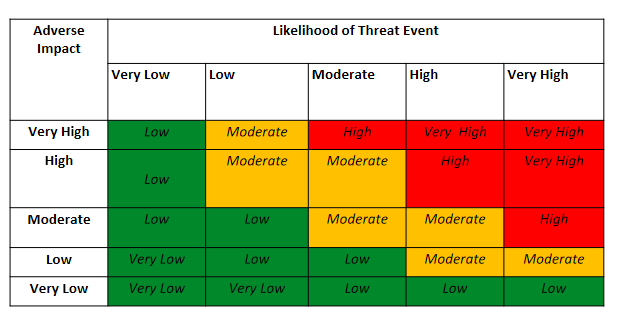
\includegraphics[width=0.8\textwidth]{images/11-7.png}
        \caption{Tabella rischio.}
        \label{fig:11-3}
    \end{figure}
\end{itemize}

\subsection{Comunicazione dei risultati}
Questa fase consiste nella produzione di un report al fine di comunicare i risultati. Lo scopo principale è comunicare i rischi più rilevanti al management e gli altri stakeholder del sistema, nonchè al personale appropriato nell'organizzazione (es: sezione IT per vulnerabilità log4j).

\subsection{Mantenimento del risk management}
L'ultima fase ha lo scopo di valutare quando rieseguire il risk assessment. Questo permette alle organizzazioni di:
\begin{itemize}
    \item Determinare l'efficacia delle risposte al rischio implementate;
    \item Identificare cambiamenti ai rischi che minacciano l'organizzazione;
    
\end{itemize}
























